\section{Evaluation}\label{sec:eval}

We implemented $\tool$ as an open-source tool~\footnote{The link is anonymized
because of a double-blind review process} in Scala by extending $\jiset$, a
JavaScript IR-based semantics extraction toolchain, with a worklist-based
fixpoint algorithm for type analysis.  Since $\jiset$ cannot automatically
compiles algorithm steps written in an uncommon writing style to $\ires$
instructions, our tool only reports type-related specification bugs detected in
fully compiled abstract algorithms.  For built-in libraries, we only targeted
abstract algorithms of essential built-in objects: \jscode{Array},
\jscode{Object}, \jscode{Function}, \jscode{Math}, \jscode{Proxy}, and objects
for primitive types.

To evaluate $\tool$, we answer the following research questions:
\begin{itemize}
  \item RQ1. \textbf{(Performance)} How long does $\tool$ take to perform type
    analysis for JavaScript specifications?
  \item RQ2. \textbf{(Precision)} How many type-related specification bugs
    detcted by $\tool$ are true bugs?
  \item RQ3. \textbf{(Effect of Refinement)} Does the condition-based refinement
    improve the analysis precision with endurable performance degradation?
  \item RQ4: \textbf{(Detection of New Bugs)} Does $\tool$ detect new
    specification bugs in the latest version of ECMAScript?
\end{itemize}
The draft of the next version of ECMAScript (ES12, 2021) is fixed on March 9,
2021.  Thus, we targeted all different 864 versions existed in the official
ECMAScript repository~\footnote{https://github.com/tc39/ecma262} for the recent
three years from January 1, 2018 to March 9, 2021.  We performed our experiments
on five Ubuntu machines equipped with 4.2GHz Quad-Core Intel Core i7 and 32GB of
RAM.


\subsection{Performance}\label{sec:performance}

Figure~\ref{fig:stat} shows four statistics of type analysis using $\tool$ for
864 versions of ECMAScript: (a) the number of analyzed functions, (b) the number
of flow- and type-sensitive views, (c) the number of worklist iterations, and
(d) the analysis time.  For each version of ECMAScript, \inred{1,999.9}
functions (\stextsf{func}) are analyzed and \inred{1,999.9} functions among them
are fully compiled (\stextsf{full-func}) on average.  Since the compile rules in
$\jiset$ is more suitable for recent versions, the number of fully compiled
functions in older versions are less than in more recent versions.  $\tool$
keeps different abstract environments for each functions divided by flow- and
type-sensitive views.  In the analysis result, \inred{1.3}M views existed for
each version and \inred{1.3}K views existed for each function on average.

We measured performance of $\tool$ based on the number of iterations for
worklist algorithm and the analysis time.  For each version of ECMAScript,
$\tool$ took \inred{300.0} seconds with \inred{19,999.9} iterations of worklist
algorithm on average.  The analysis time consists of \inred{10.0} seconds for
the specification extraction (\stextsf{extract} with gray bars), \inred{340.0}
seconds for the type analysis (\stextsf{analyze} with blue bars), \inred{10.0}
seconds for the bug detection (\stextsf{detect} with red bars).


\subsection{Precision}\label{sec:precision}

\begin{table}
  \centering
  \caption{The creators and resolvers of true bugs.}
  \label{table:author}
  \resizebox{\columnwidth}{!}{%
  \begin{tabular}{c|c|c?c|c|c}
    \multicolumn{3}{c?}{\textbf{Creator}} &
    \multicolumn{3}{c}{\textbf{Resolver}}\\\hline

    \textbf{Committee} &
    \textbf{Outsider} &
    \textbf{Inherited} &
    \textbf{Committee} &
    \textbf{Outsider} &
    \textbf{NotYet}\\\hline

    \inred{60} &
    \inred{12} &
    \inred{20} &
    \inred{60} &
    \inred{23} &
    \inred{10}\\
  \end{tabular}
  }
  \vspace*{-1.5em}
\end{table}

\begin{figure}
  \centering
  \begin{subfigure}[b]{0.24\textwidth}
    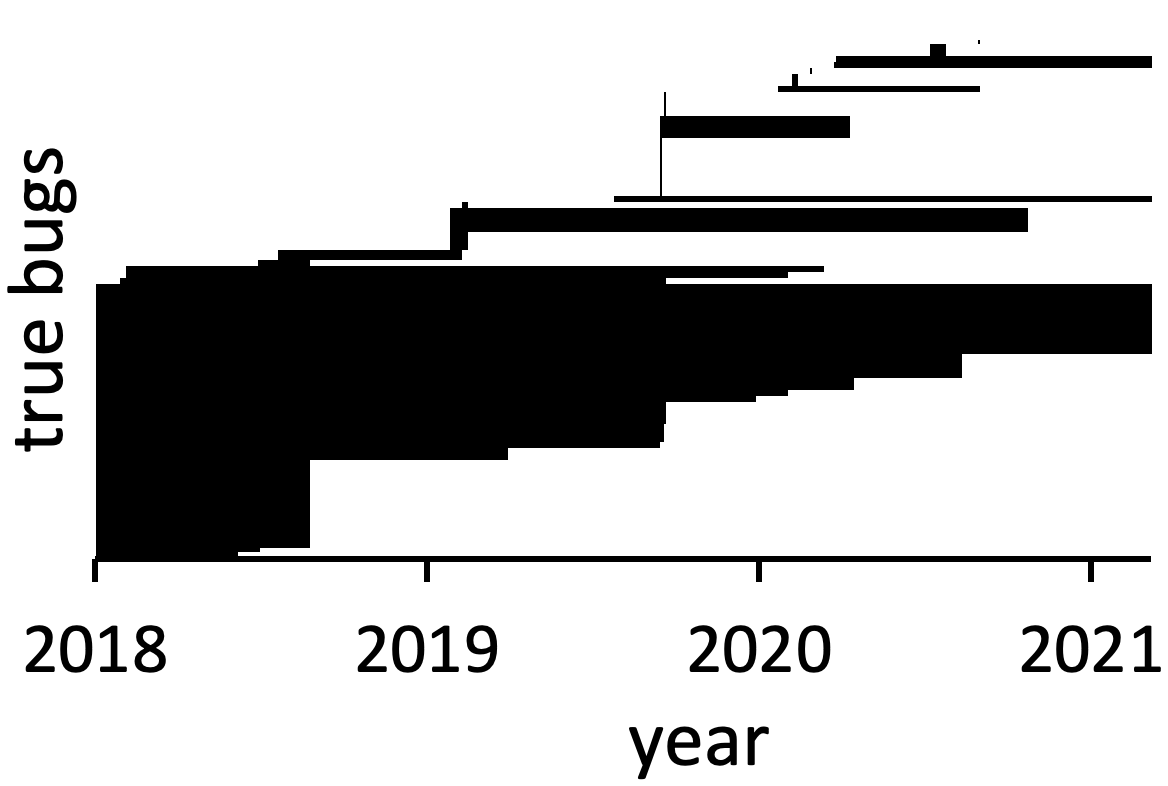
\includegraphics[width=\textwidth]{img/ttl-chro}
    \caption{TTLs sorted by creation time.}
  \end{subfigure}
  \begin{subfigure}[b]{0.24\textwidth}
    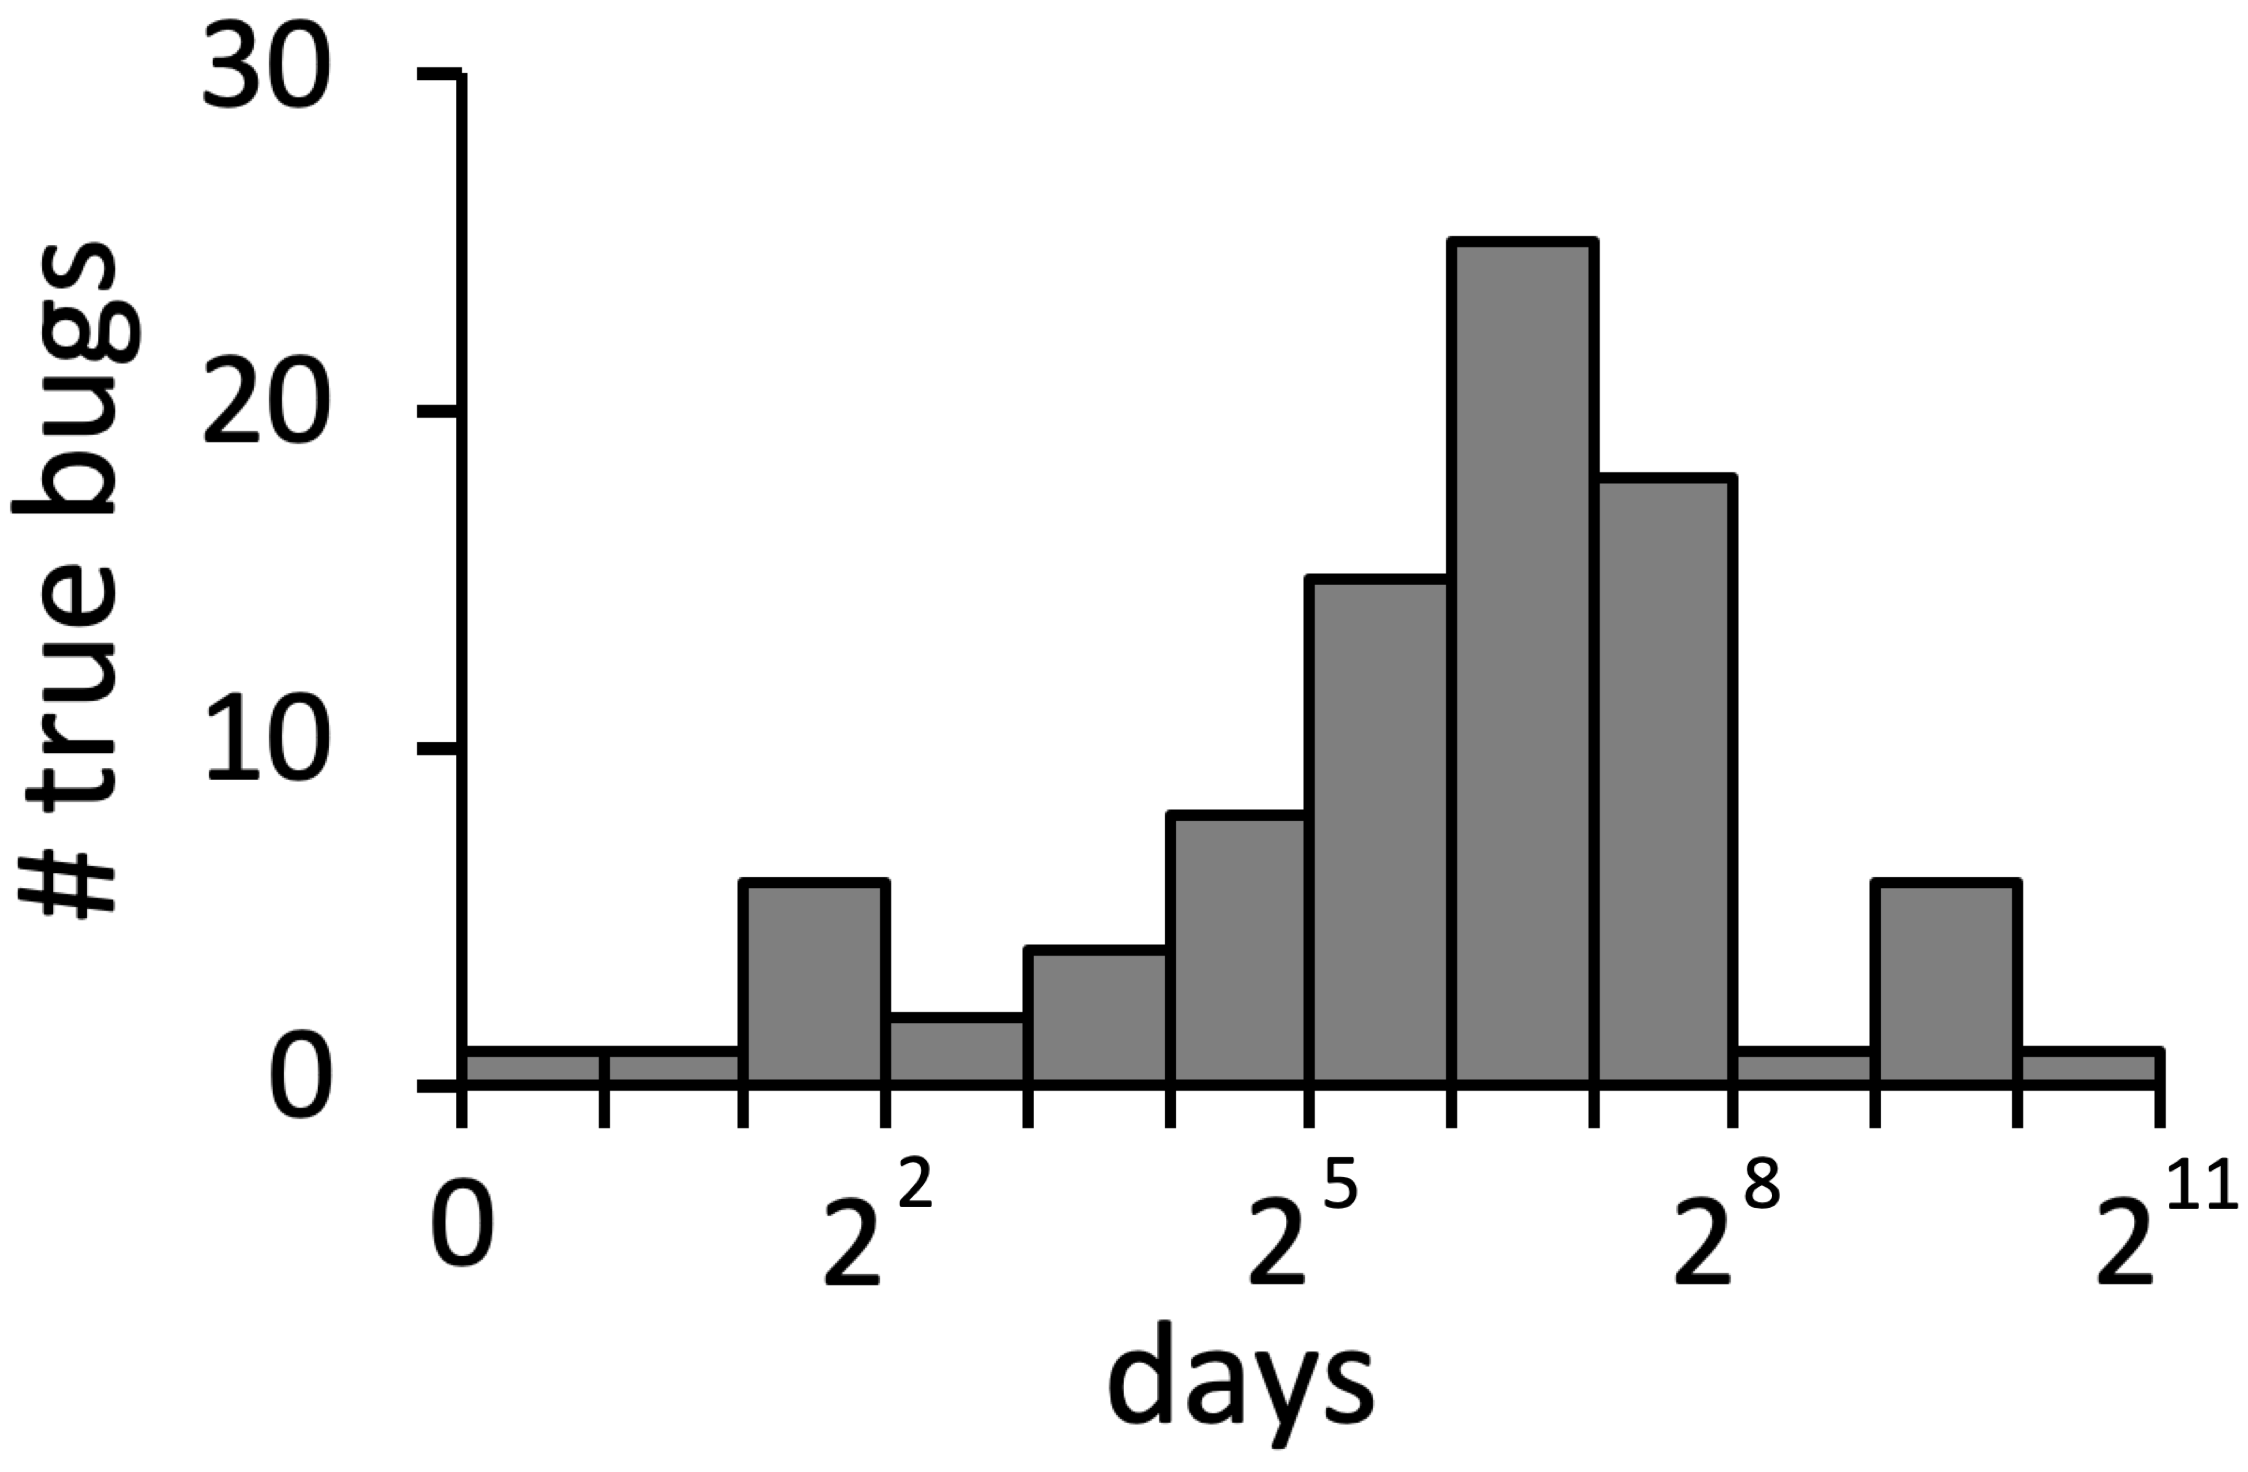
\includegraphics[width=\textwidth]{img/ttl-count}
    \caption{The histogram of TTLs.}
  \end{subfigure}
  \caption{Time to Lives (TTLs) of true bugs.}
  \vspace*{-1.5em}
  \label{fig:ttl}
\end{figure}

\begin{table*}
  \centering
  \caption{The analysis precision of $\tool$ without refinement
  (\stextsf{no-refine}), with refinement (\stextsf{refine}), and their
  difference ($\Delta$)}
  \label{table:precision}
  \resizebox{\textwidth}{!}{%
  \begin{tabular}{c|c?c|c?c|c?c|c}
    \multirow{2}{*}{\textbf{Checker}} &
    \multirow{2}{*}{\textbf{Bug Kind}} &
    \multicolumn{6}{c}{
      \textbf{Precision = (\# True Bugs) / (\# Detected Bugs)}
    }\\\cline{3-8} &&
    \multicolumn{2}{c?}{no-refine} &
    \multicolumn{2}{c?}{refine} &
    \multicolumn{2}{c}{$\Delta$}\\

    \specialrule{.1em}{.0em}{.0em}

    \myrowc{2}
    {Reference}     {60 / 116 (51.7\%)} {60 / 116 (51.7\%)} {\md{12}{3}{51.7}}
    {UnknownVar}    {17 / 72 (23.6\%)}  {17 / 72 (23.6\%)}  {\md{12}{3}{51.7}}
    \myrowh
    {DuplicatedVar} {43 / 44 (97.7\%)}  {43 / 44 (97.7\%)}  {\md{12}{3}{51.7}}

    \hline

    \myrowc{1}
    {Arity}         {60 / 116 (51.7\%)} {60 / 116 (51.7\%)} {\md{12}{3}{51.7}}
    {MissParam}     {17 / 72 (23.6\%)}  {17 / 72 (23.6\%)}  {\md{12}{3}{51.7}}

    \hline

    \myrowc{1}
    {Assertion}     {60 / 116 (51.7\%)} {60 / 116 (51.7\%)} {\md{12}{3}{51.7}}
    {Assertion}     {17 / 72 (23.6\%)}  {17 / 72 (23.6\%)}  {\md{12}{3}{51.7}}

    \hline

    \myrowc{2}
    {Operand}       {60 / 116 (51.7\%)} {60 / 116 (51.7\%)} {\md{12}{3}{51.7}}
    {NoNumber}      {17 / 72 (23.6\%)}  {17 / 72 (23.6\%)}  {\md{12}{3}{51.7}}
    \myrowh
    {Abrupt}        {43 / 44 (97.7\%)}  {43 / 44 (97.7\%)}  {\md{12}{3}{51.7}}

    \specialrule{.1em}{.0em}{.0em}

    \mysrowh
    {\textbf{Total}}{43 / 44 (97.7\%)}  {43 / 44 (97.7\%)}  {\md{12}{3}{51.7}}

  \end{tabular}
  }
  \vspace*{-1.5em}
\end{table*}


We measured the analysis precision based on the number of true bugs in
type-related specification bugs detected by $\tool$.  As described in the
\stextsf{refine} column of Table~\ref{table:precision}, the analysis precision
is \inred{51.7}\% because it detected \inred{190} type-related bugs and
\inred{89} bugs are true bugs among them.  The reference checker detected the
largest number of bugs with \inred{51.7}\% precision; it found \inred{12} true
reference bugs for \inred{32} unknown variables (\stextsf{UnknownVar}) and
\inred{32} already defined variables (\stextsf{DuplicatedVar}). The arity
checker and the assertion checker found \inred{12} missing parameters
(\stextsf{MissParam}) with \inred{90.2}\% precision and \inred{12} assertion
failures (\stextsf{Assertion}) with \inred{90.2}\% precision, respectively.
Finally, the operand checker detected two different kinds of wrong typed operand
bugs: \inred{12} non-numeric operand bugs (\stextsf{NoNumber}) for numeric
operators with \inred{12.3}\% precision and \inred{12} unchecked abrupt
completion bugs (\stextsf{Abrupt}) with \inred{12.3}\% precision.

Moreover, we extended $\tool$ to automatically extract more statistics of
detected true bugs.  \inred{First, we checked that true bugs are created or
resolved by whom as described in Table~\ref{table:author}.  Among \inred{89}
true bugs, we cannot automatically know who created \inred{20}
\textit{inherited} bugs, which are created before 2018.  For remaining
\inred{20} bugs, only \inred{20} bugs are created by members of the Ecma
Technical Committee 39 (TC39) but others (\inred{20} bugs) are created by
outside contributors not committee members.  On the other hand, most of them
(\inred{20} bugs) are resolved by the committee members but only \inred{20} bugs
are resolved by non-committee contributors.  Other \inred{14} bugs are newly
found and we will explain their details in Section~\ref{sec:new-bug}.}  Another
statistic of true bugs is Time to Live (TTL) that denotes how many days
specification bugs existed.  Figure~\ref{fig:ttl} describes TTLs of true bugs;
the left chart (Figure~\ref{fig:ttl}(a)) depicts their periods sorted by their
creation time, and the right chart (Figure~\ref{fig:ttl}(b)) depicts the
histogram of TTLs in a logarithmic scale.  The average days of TTL is
\inred{300.0} even though we assume that \inred{20} inherited bugs are created
in January 1, 2018.  The maximum length of TTL is \inred{1,000} and the
corresponding bug is inherited and not yet resolved in the latest version.  We
manually investigated its creation time in the history of the official
repository, and we discovered that it was created at the initial commit of the
open development process in September 22, 2015.  It means that the bug actually
existed for \inred{3,000} days.


\subsection{Effectiveness of Refinement}\label{sec:effect-refine}

\begin{table*}
  \centering
  \caption{Type-related specification bugs newly detected by $\tool$ in the
  official draft of ECMAScript 2021 (ES12).}
  \label{table:new-bug}
  \resizebox{\textwidth}{!}{%
  \begin{tabular}{@{}c@{~}?c|@{~}c@{~}|l|c|@{~}c@{~}|@{~}c@{~}|@{~}r@{}}
    \multicolumn{1}{@{}c?}{\textbf{Name}} &
    \multicolumn{1}{c}{\textbf{Feature}} &
    \multicolumn{1}{@{}c@{~}}{\textbf{\#}} &
    \multicolumn{1}{c}{\textbf{Description}} &
    \multicolumn{1}{@{~}c@{~}}{\textbf{Checker}} &
    \multicolumn{1}{@{}c}{\textbf{Created}} &
    \multicolumn{1}{@{}c}{\textbf{Resolved}} &
    \multicolumn{1}{@{}c@{~}}{\textbf{TTL}}\\\specialrule{.1em}{.0em}{.0em}

    ES12-1 &
    Switch &
    3 &
    \makecell[l]{
        Variables \code{hasDuplicates} and \code{hasUndefinedLabels} are already \\
        defined in algorithms for \jscode{case} blocks of \jscode{switch}
        statements.
    } &
    \stextsf{Reference} &
    \inred{2015-01-01} &
    \inred{2015-01-01} &
    \inred{1,999} days\\\hline

    ES12-2 &
    Try &
    3 &
    \makecell[l]{
        Variables \code{hasDuplicates} and \code{hasUndefinedLabels} are already \\
        defined in algorithms for \jscode{try} statements.
    } &
    \stextsf{Reference} &
    \inred{2015-01-01} &
    \inred{2015-01-01} &
    \inred{1,999} days\\\hline

    ES12-3 &
    Arguments &
    1 &
    \makecell[l]{
        A variable \code{index} is already defined in
        \textbf{CreateMappedArgumentsObject}.
    } &
    \stextsf{Reference} &
    \inred{2015-01-01} &
    \inred{2015-01-01} &
    \inred{1,999} days\\\hline

    ES12-4 &
    Array &
    2 &
    \makecell[l]{
        A variable \code{succeeded} is already defined in algorithms for
        \jscode{Array} objects.
    } &
    \stextsf{Reference} &
    \inred{2015-01-01} &
    \inred{2015-01-01} &
    \inred{1,999} days\\\hline

    ES12-5 &
    Async &
    1 &
    \makecell[l]{
        A variable \code{value} is already defined in \textbf{Evaluation} for
        \jscode{yield} expressions.
    } &
    \stextsf{Reference} &
    \inred{2015-01-01} &
    \inred{2015-01-01} &
    \inred{1,999} days\\\hline

    ES12-6 &
    Class &
    1 &
    \makecell[l]{
        A variable \code{ClassHeritage} is not defined in \textbf{Contains}
        \\ for tails of \jscode{class} declarations.
    } &
    \stextsf{Reference} &
    \inred{2015-01-01} &
    \inred{2015-01-01} &
    \inred{1,999} days\\\hline

    ES12-7 &
    Branch &
    1 &
    \makecell[l]{
        A variable \code{Statement} is not defined in \textbf{EarlyErrors} for
        \jscode{if} statement.
    } &
    \stextsf{Reference} &
    \inred{2015-01-01} &
    \inred{2015-01-01} &
    \inred{1,999} days\\\hline

    ES12-8 &
    Arguments &
    2 &
    \makecell[l]{
        Abrupt completions are used in \textbf{DefineOwnProperty} and
        \textbf{GetOwnProperty} \\ for \jscode{arguments} objects without any
        checks.
    } &
    \stextsf{Operand} &
    \inred{2015-01-01} &
    \inred{2015-01-01} &
    \inred{1,999} days\\
  \end{tabular}
  }
  \vspace*{-1.5em}
\end{table*}

\begin{figure}
  \centering
  \begin{subfigure}[b]{0.24\textwidth}
    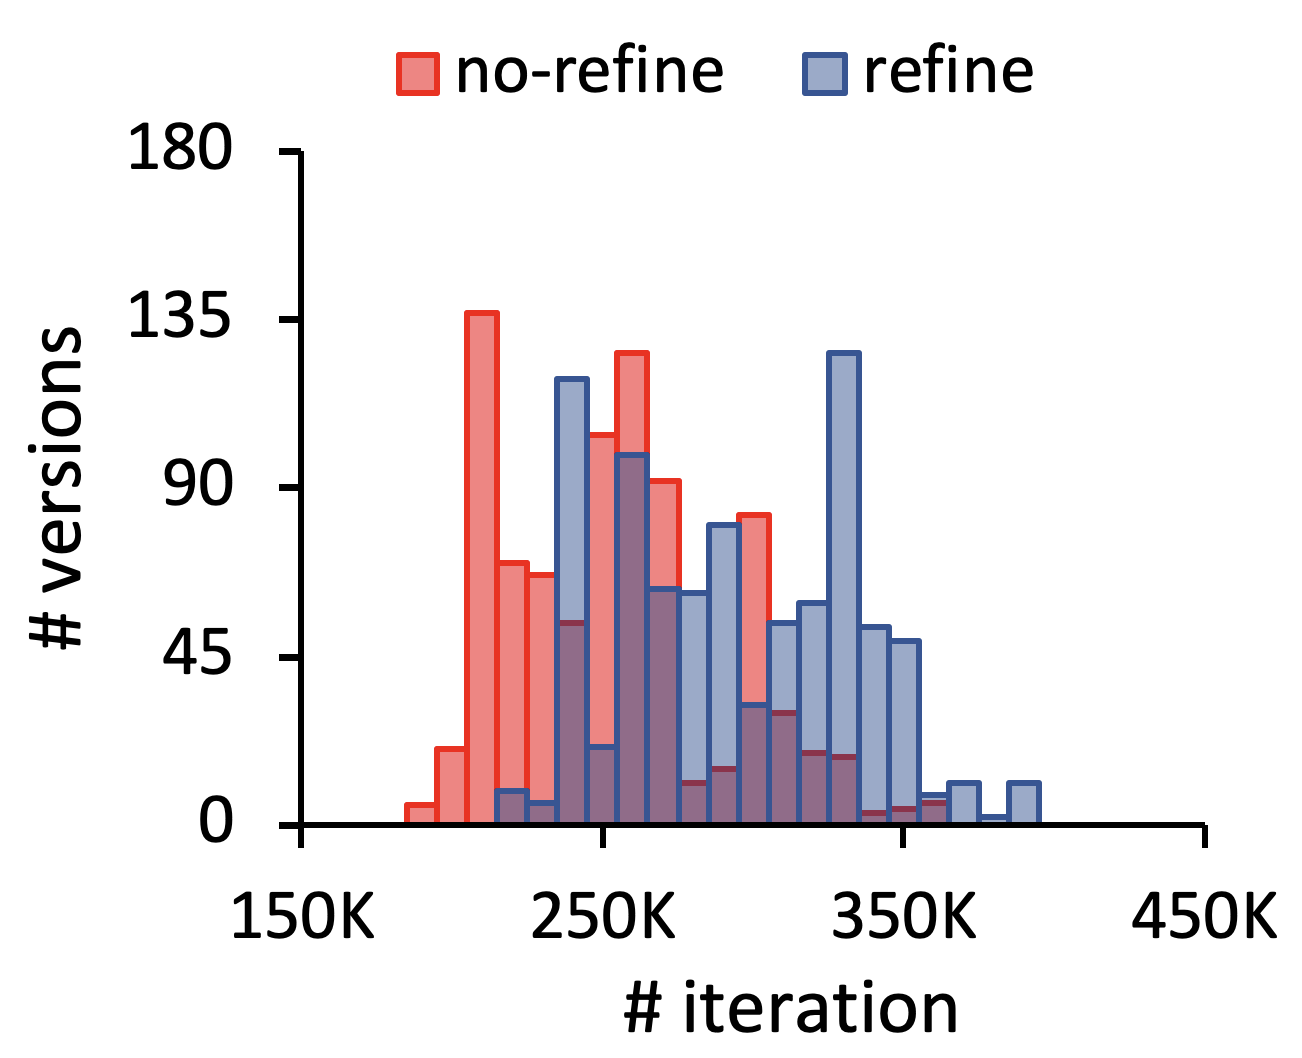
\includegraphics[width=\textwidth]{img/compare-iter}
    \caption{The histogram of iterations.}
  \end{subfigure}
  \begin{subfigure}[b]{0.24\textwidth}
    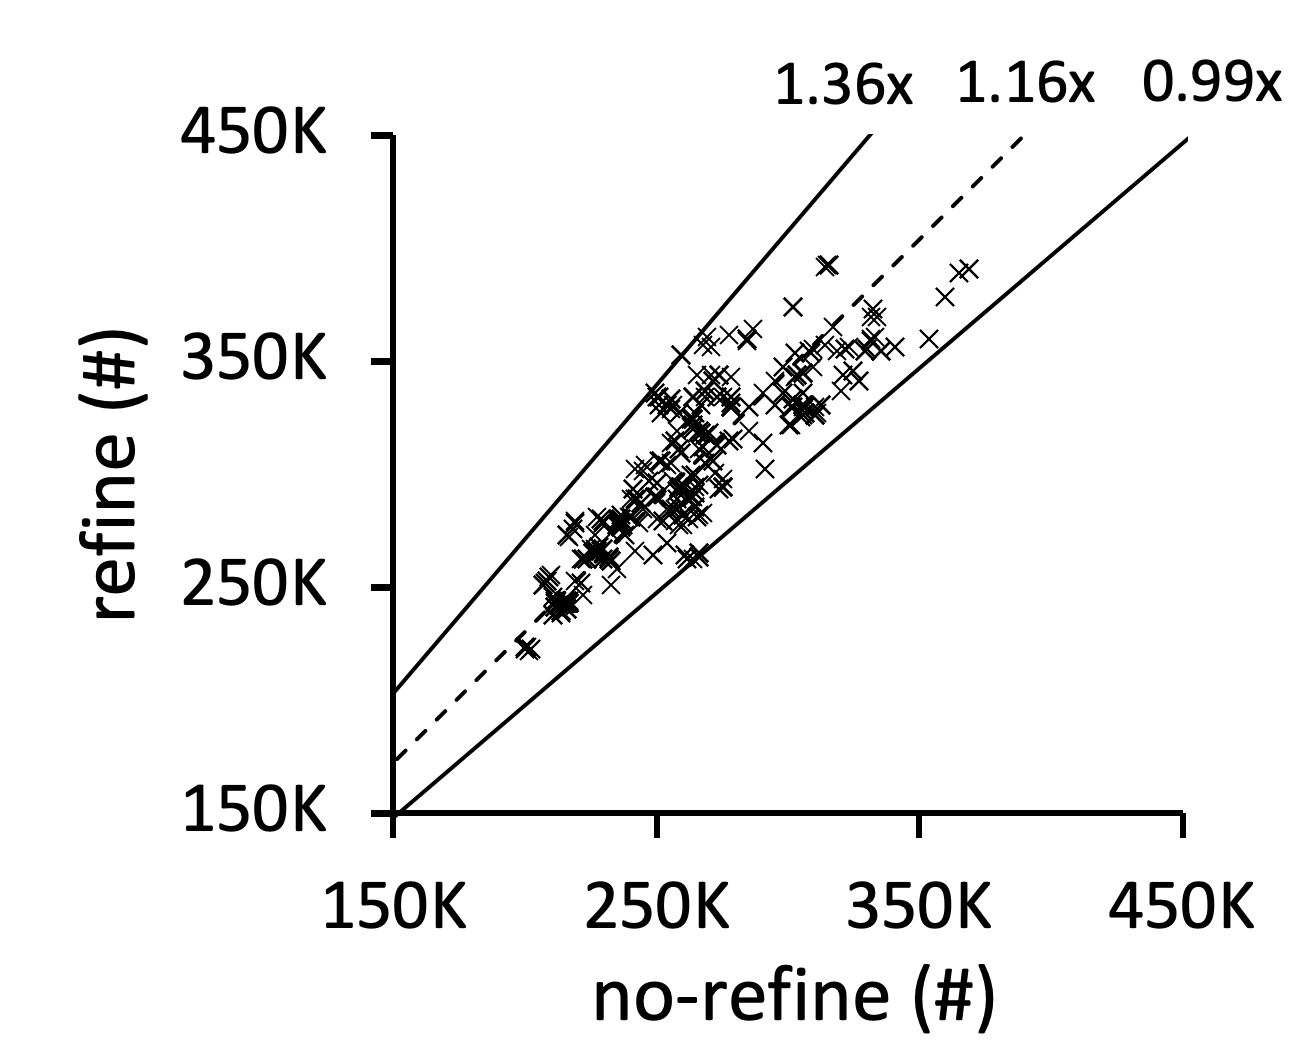
\includegraphics[width=\textwidth]{img/ratio-iter}
    \caption{The ratio of iterations.}
  \end{subfigure}
  \begin{subfigure}[b]{0.24\textwidth}
    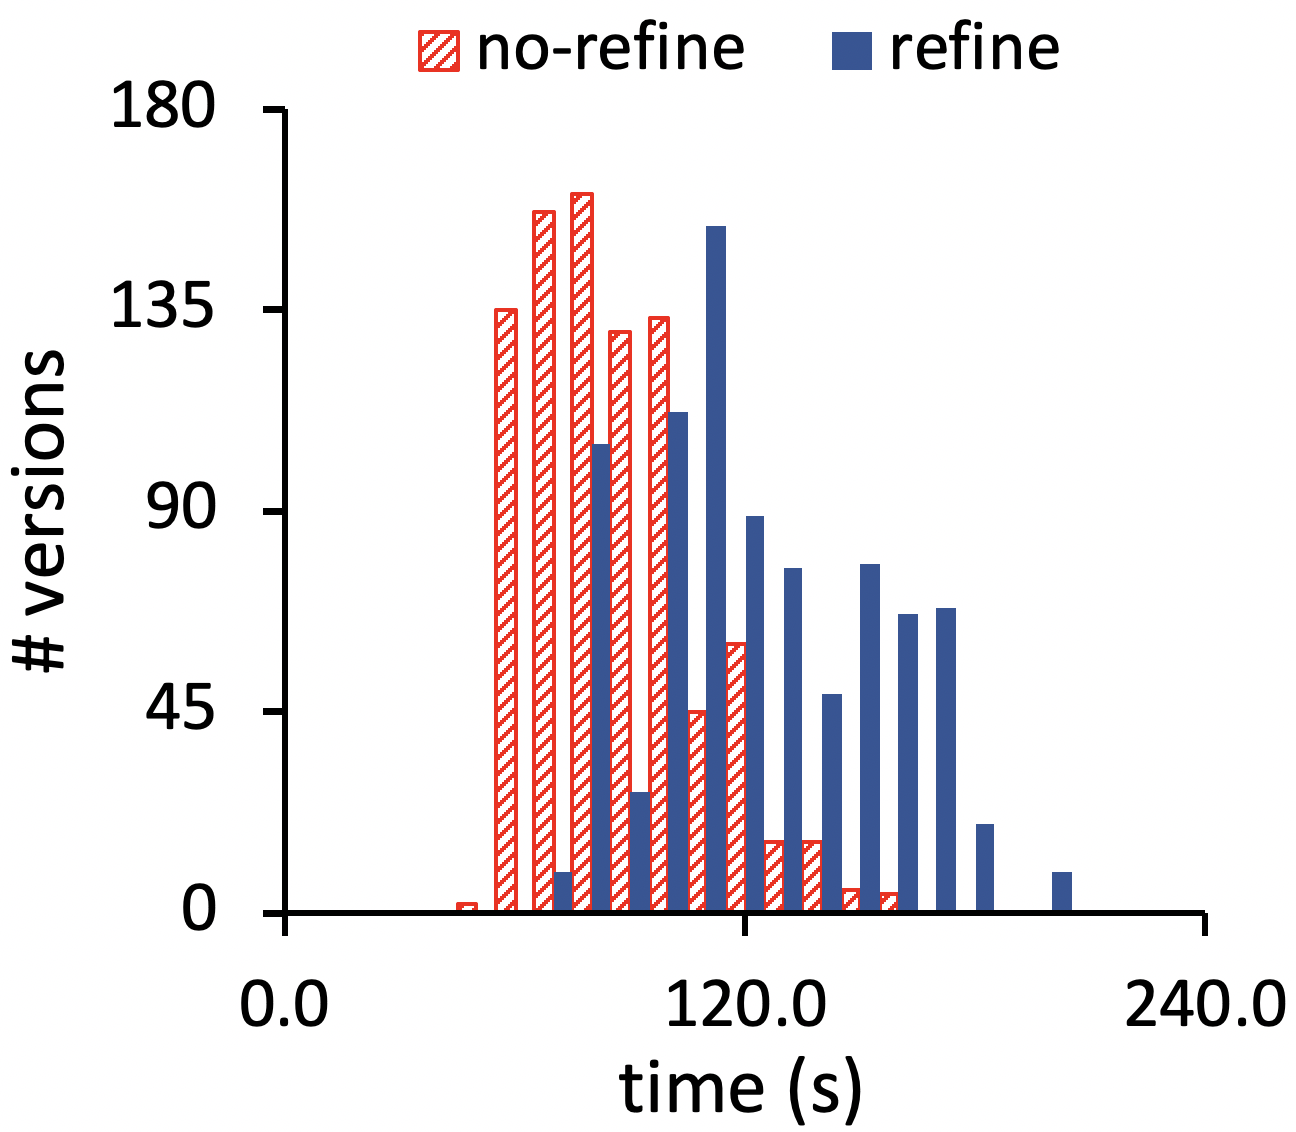
\includegraphics[width=\textwidth]{img/compare-time}
    \caption{The histogram of time.}
  \end{subfigure}
  \begin{subfigure}[b]{0.24\textwidth}
    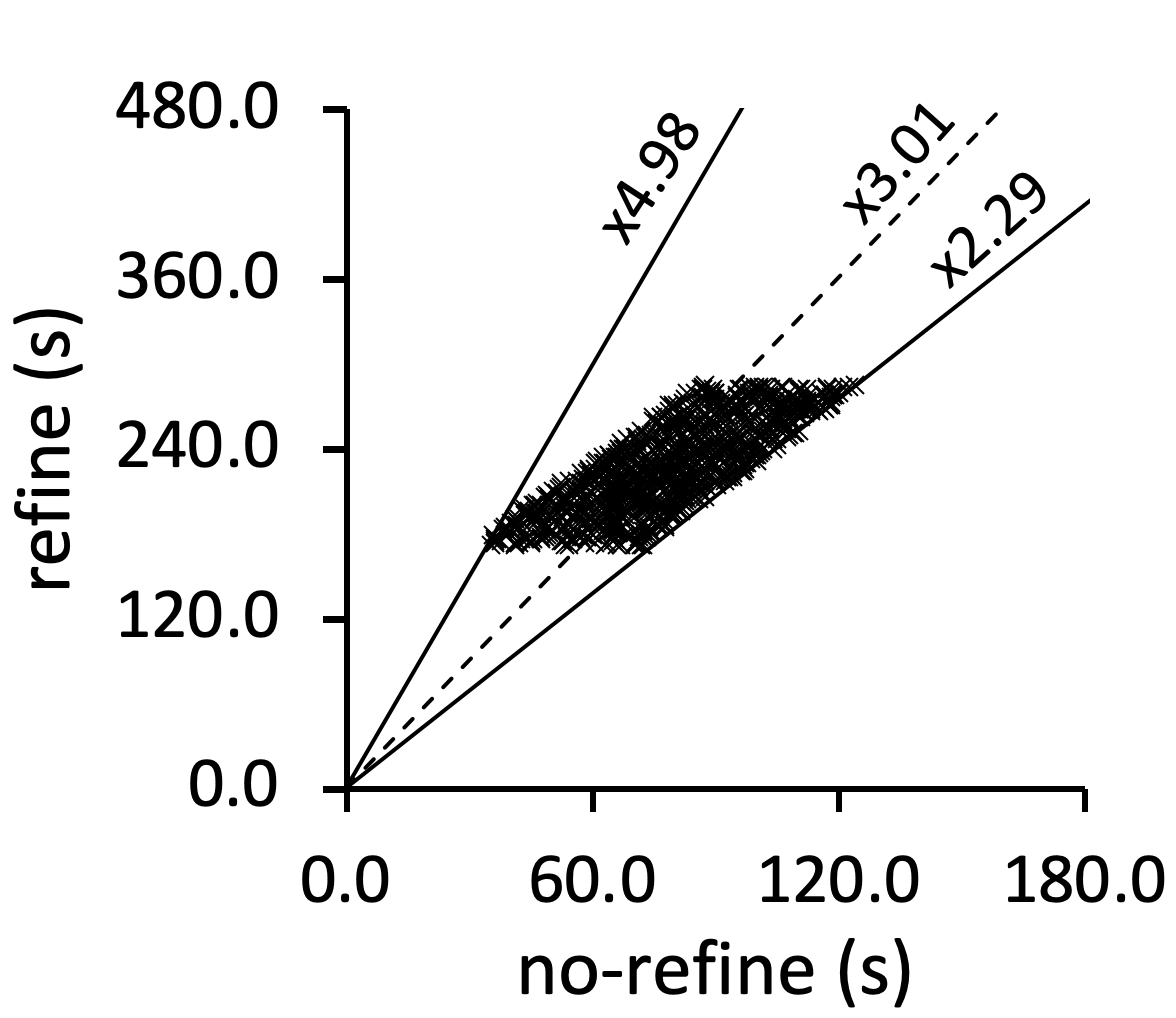
\includegraphics[width=\textwidth]{img/ratio-time}
    \caption{The ratio of time.}
  \end{subfigure}
  \caption{The comparison of iterations and analysis time without refinement
  (\stextsf{no-refine}) and with refinement (\stextsf{refine}).}
  \label{fig:performance-compare}
  \vspace*{-1.5em}
\end{figure}

We evaluated the effectiveness of condition-based refinement based on how much
it improved analysis precision without significant performance degradation.  To
compare performance and precision of analysis without refinement
(\stextsf{no-refine}) and with refinement (\stextsf{refine}), we also performed
$\tool$ without refinement for 864 versions of ECMAScript.

For performance, Figure~\ref{fig:performance-compare} describes the comparison
of iterations and analysis time without refinement and with refinement; the left
charts (Figure~\ref{fig:performance-compare}(a) and
\ref{fig:performance-compare}(c)) are histograms of iterations and analysis
time, and the right charts (Figure~\ref{fig:performance-compare}(b) and
\ref{fig:performance-compare}(d)) are scatter charts for their ratio.  Without
refinement, type analysis took \inred{234.3} seconds with \inred{232}K
iterations on average.  With refinement, it took \inred{234.3} seconds with
\inred{232}K iterations on average.  For each version, analysis time is
increased at least \inred{2.3}x, at most \inred{2.3}x, and \inred{2.3}x on
average, and the number of iterations is increased at least \inred{2.3}x, at
most \inred{2.3}x, and \inred{2.3}x on average.

Table~\ref{table:precision} shows the analysis precision without refinement,
with refinement, and their difference.  The refinement improved the analysis
precision from \inred{23.2}\% to \inred{23.3}\% by removing \inred{10} false
bugs and to detect \inred{10} more true bugs.  \inred{(\todo: investigate the result for
each checker.)}


\subsection{Detection of New Bugs}\label{sec:new-bug}

Among \inred{91} true bugs detected by $\tool$, \inred{14} bugs are newly
detected and still exist in the latestest version of ECMAScript.
Table~\ref{table:new-bug} summarizes the bugs categorized by their kinds and
related JavaScript language features. It includes their TTLs, and we manually
investigated their extact creation time if they are created before 2018.  We
reported the newly detected bugs to TC39; all of them are confirmed by the
committee and will be fixed in ECMAScript 2022 (ES13).

ES12-1 contains three bugs that are due to the duplicated definition of
variables in three different algorithms for \jscode{case} blocks of
\jscode{switch} statements: \code{hasDuplicates} in
\textbf{ContainsDuplicateLabels}, and \code{hasUndefinedLabels} in
\textbf{ContainsUndefinedBreakTarget} and
\textbf{ContainsUndefinedContinueTarget}.  Each \jscode{case} block optionally
contains \jscode{case} clauses, and three algorithms perform additional stpes
including to define \code{hasDuplicates} (or \code{hasUndefinedLabels}) when the
clauses exist at the beginning.  However, the exactly same variable is defined
again after the coditionally additional steps.  It means that the semantics of
\jscode{case} blocks having \jscode{case} clauses always have reference for
already defined variable \code{hasDuplicates} (or \code{hasUndefinedLabels}).
ES12-2 also contains three bugs caused by the exactly same reasons in same
abstract algorithms for \jscode{try} statements.

The bug in ES12-3 is a reference bug for already defined variable \code{index}
in the abstract algorithm \textbf{CreateMappedArgumentsObject}.  For each
function call in JavaScript programs, an \jscode{arguments} object is created by
\textbf{CreateMappedArgumentsObject}.  In the algorithm, the variable
\code{index} is defined to handle the index of a given list of arguments.
However, the variable is defined twice in step 14 and 17 of the algorithm.

ES12-4 contains two reference bugs for already defined variable \code{succeeded}
in \textbf{DefineOwnProperty} of \jscode{Array} objects and
\textbf{ArraySetLength}.  The \jscode{Array} objects are exotic, which means
that they are not ordinay objects and have special algorithms for specific
behaviors.  The two algorithms are wrapper algorithms of
\textbf{OrdinaryDefineOwnProperty} which updates object properties.  They define
the variable \code{succeeded} to represent the result of
\textbf{OrdinaryDefineOwnProperty}.  However, the variable is defined twice in a
specific condition.

The bug in ES12-5 is a reference bug for already defined variable \code{value}
in \textbf{Evaluation} of defined \jscode{yield} expressions.  In the evaluation
of \jscode{yield * e}, the variable \code{value} is defined twice to
represent 1) the evaluation result of the given expression \jscode{e} in step
3, and 2) to the iterator value in step 7.c.viii.1.

The bug in ES12-6 is a reference bug for unknown variable \code{ClassHeritage}
in \textbf{Contains} for tails of \jscode{class} declarations.  A tail of
\jscode{class} declaration consists of an optional class heritage with
\jscode{extneds} keyword and a class body enclosed by curly braces.  When the
optional class heritage does not exist, the variable \code{ClassHeritage} is not
defined but the \textbf{Contains} algorithm tries to access it without any check
of its existence.

The bug in ES12-7 is a reference bug for unknown variable \code{Statement} in
\textbf{EarlyErrors} for \jscode{if} statements.  In syntax-directed algorithms,
the ordinal numbers are used as prefixes of variables when multiple sub-ASTs are
produced by same productions.  A \jscode{if} statement contains two sub-ASTs
produced by the \textit{Statement} production thus the ordinal number prefixes
are required for the variable \code{Statement}.  However, the
\textbf{EarlyErrors} algorithm for \jscode{if} statements uses it without any
ordinal number prefixes.

ES12-8 contains two operand type bugs related to abrupt completions in
\textbf{DefineOwnProperty} and \textbf{GetOwnProperty} for \jscode{arguments}
objects.  The two algorithms define or get own properties of \jscode{arguments}
exotic objects.  They utilize the \textbf{Get} algorithm that returns JavaScript
values stored in object properties or abrupt completions.  Thus, they should
check whether results of \textbf{Get} are abstract completions or not before
using them.  However, they use the results without any abrupt completion checks.
